\documentclass[12pt]{article}
\usepackage{setspace, graphicx, fullpage, amssymb, amsmath, epsfig, natbib, array, multirow, hyperref}
\usepackage{amsfonts, bm} 
\usepackage{dcolumn}
\usepackage{subfigure, float} 
\usepackage[margin=1in]{geometry} 
\usepackage{verbatim}
\usepackage{url}
\usepackage{enumerate}
\newcolumntype{d}[1]{D{.}{.}{#1}} 

\begin{document}

\begin{center}
\Large 22 February 2017
\end{center}

\section{Overview}

The main tasks I set out to accomplish over week as per our last meeting were as follows:

\begin{itemize}
	\item Continue showing differences between the OLS/\verb|lm| and the bias-reduced logit/\verb|brglm| sorting algorithms

	\item Explore the trade off of coefficients between party and ideology in the vote sorting algorithm
\end{itemize}

\noindent
Craig had previously expressed concerns with the sorting of votes on two fronts; the first being that the algorithm using the bias-reduced logistic equation for sorting votes was largely not sorting close votes as party votes and the second that it could mean very different things to have a vote sorted as a party vote when the equation has opposite signs on the coefficients for party and ideology than when these are the same. On the latter category, William hypothesized instead that it could be evidence of party pressure overcoming ideology when the direction is opposite, which would leave it more in line with the basic theory and work we have been doing up until this point. While it was agreed that we would look into the results from the algorithm, William had suggested saving analysis of coefficients for a later project and focusing on extending analysis into the Senate.

The information I show below shows the information previously given for other versions of the model for the House and Senate \verb|lm| sorted algorithm. We should discuss any final thoughts we have regarding the different sorting algorithms as well as what we should make of the signs on the coefficients now or at a later date. Depending on what is decided, it may be wise to think about next steps for the project should be and how we wish to pursue them.

\pagebreak

\section{Tables and Figures}

This part of the update will contain the Senate tables and figures, with the House tables and figures included in a second document.

\subsection{Senate lm Descriptive Statistics}

% latex table generated in R 3.3.2 by xtable 1.8-2 package
% Mon Feb 20 16:00:02 2017
\begin{table}[ht]
	\centering
	\caption{Coding by Congress}
	\begin{tabular}{rrrr}
		\hline
		congress & party calls & noncalls & gray votes \\ 
		\hline
		93 & 417 & 611 &   2 \\ 
		94 & 456 & 745 &   2 \\ 
		95 & 332 & 765 &   3 \\ 
		96 & 412 & 562 &   1 \\ 
		97 & 465 & 393 &   2 \\ 
		98 & 316 & 280 &   0 \\ 
		99 & 305 & 390 &   4 \\ 
		100 & 356 & 328 &   2 \\ 
		101 & 263 & 272 &   1 \\ 
		102 & 278 & 219 &   4 \\ 
		103 & 396 & 272 &   3 \\ 
		104 & 528 & 300 &   0 \\ 
		105 & 298 & 233 &   3 \\ 
		106 & 378 & 213 &   5 \\ 
		107 & 289 & 202 &   7 \\ 
		108 & 380 & 176 &   0 \\ 
		109 & 332 & 211 &   1 \\ 
		110 & 331 & 252 &   5 \\ 
		111 & 490 & 147 &   1 \\ 
		112 & 274 & 156 &  10 \\ 
		\hline
		Total: & 7296 & 6727 & 56 \\
		Mean & 364.8 & 336.4 & 2.8 \\
		sd: & 77.0 & 187.9 & 2.5 \\
		\hline
	\end{tabular}
\end{table}

% latex table generated in R 3.3.2 by xtable 1.8-2 package
% Mon Feb 20 16:03:06 2017
\begin{table}[ht]
	\centering
	\caption{Coding by Close/Lopsided}
	\begin{tabular}{rrrr}
		\hline
		& party call & noncall & gray \\ 
		\hline
		lopsided & 2063 & 4876 &  47 \\ 
		close & 5233 & 1851 &   9 \\ 
		\hline
	\end{tabular}
\end{table}



% Table created by stargazer v.5.2 by Marek Hlavac, Harvard University. E-mail: hlavac at fas.harvard.edu
% Date and time: Mon, Feb 20, 2017 - 20:49:00
\begin{table}[!htbp] \centering 
	\caption{Responsiveness Statistics} 
	\label{} 
	\begin{tabular}{@{\extracolsep{5pt}}lccccc} 
		\\[-1.8ex]\hline 
		\hline \\[-1.8ex] 
		Statistic & \multicolumn{1}{c}{N} & \multicolumn{1}{c}{Mean} & \multicolumn{1}{c}{St. Dev.} & \multicolumn{1}{c}{Min} & \multicolumn{1}{c}{Max} \\ 
		\hline \\[-1.8ex] 
		Democrats: & & & & & \\
		\hline
		party free ideal point & 1,043 & $-$0.656 & 0.658 & $-$3.222 & 1.630 \\ 
		pirate100 & 1,043 & 85.789 & 10.890 & 8.777 & 100.000 \\ 
		pfrate100 & 1,042 & 83.760 & 7.862 & 45.106 & 100.000 \\ 
		ideological extremism & 1,043 & 0.656 & 0.658 & $-$1.630 & 3.222 \\ 
		\hline
		Republicans: & & & & & \\
		\hline
		party free ideal point & 951 & 0.725 & 0.789 & $-$1.595 & 3.397 \\ 
		pirate100 & 951 & 85.180 & 12.011 & 33.232 & 100.000 \\ 
		pfrate100 & 951 & 80.144 & 8.073 & 50.070 & 100.000 \\ 
		ideological extremism & 951 & 0.725 & 0.789 & $-$1.595 & 3.397 \\ 
		\hline
		Majority Party: & & & & & \\
		\hline
		party free ideal point & 1,053 & $-$0.070 & 0.918 & $-$1.966 & 2.866 \\ 
		pirate100 & 1,053 & 86.946 & 10.353 & 37.020 & 100.000 \\ 
		pfrate100 & 1,052 & 83.089 & 8.216 & 45.106 & 100.000 \\ 
		ideological extremism & 1,053 & 0.613 & 0.687 & $-$1.630 & 2.866 \\ 
		\hline
		Minority Party: & & & & & \\
		\hline
		party free ideal point & 843 & 0.091 & 1.086 & $-$3.222 & 3.397 \\ 
		pirate100 & 843 & 83.138 & 12.372 & 8.777 & 100.000 \\ 
		pfrate100 & 843 & 80.354 & 8.068 & 50.070 & 100.000 \\ 
		ideological extremism & 843 & 0.767 & 0.773 & $-$1.269 & 3.397 \\ 
		\hline \\[-1.8ex] 
	\end{tabular} 
\end{table} 

\pagebreak

\subsection{Senate lm Models}

\begin{table}
	\begin{center}
		\caption{Bivariate DV/IV Regressions}
		\begin{tabular}{l c c c c }
			\hline
			& Democrats & Democrats & Republicans & Republicans \\
			\hline
			pfrate100              & $1.06^{***}$ &               & $0.92^{***}$  &               \\
			& $(0.03)$     &               & $(0.04)$      &               \\
			ideological extremism &              & $10.05^{***}$ &               & $8.90^{***}$  \\
			&              & $(0.41)$      &               & $(0.40)$      \\
			(Intercept)            & $-2.85$      & $79.19^{***}$ & $11.55^{***}$ & $78.73^{***}$ \\
			& $(2.33)$     & $(0.38)$      & $(3.06)$      & $(0.43)$      \\
			\hline
			R$^2$                  & 0.58         & 0.37          & 0.38          & 0.34          \\
			Adj. R$^2$             & 0.58         & 0.37          & 0.38          & 0.34          \\
			Num. obs.              & 1042         & 1043          & 951           & 951           \\
			RMSE                   & 7.03         & 8.66          & 9.45          & 9.75          \\
			\hline
			\multicolumn{5}{l}{\scriptsize{$^{***}p<0.001$, $^{**}p<0.01$, $^*p<0.05$}}
		\end{tabular}
	\end{center}
\end{table}

\begin{table}
	\begin{center}
		\caption{Multivariate DV/IV Regressions}
		\begin{tabular}{l c c c c }
			\hline
			& Democrats & Republicans & Majority & Minority \\
			\hline
			pfrate100              & $0.849^{***}$  & $0.774^{***}$  & $0.727^{***}$  & $0.717^{***}$  \\
			& $(0.030)$      & $(0.031)$      & $(0.025)$      & $(0.036)$      \\
			ideological extremism & $4.727^{***}$  & $7.289^{***}$  & $5.570^{***}$  & $7.748^{***}$  \\
			& $(0.362)$      & $(0.319)$      & $(0.304)$      & $(0.371)$      \\
			(Intercept)            & $11.566^{***}$ & $17.872^{***}$ & $23.150^{***}$ & $19.552^{***}$ \\
			& $(2.426)$      & $(2.474)$      & $(2.050)$      & $(2.797)$      \\
			\hline
			R$^2$                  & 0.643          & 0.601          & 0.648          & 0.590          \\
			Adj. R$^2$             & 0.642          & 0.600          & 0.647          & 0.589          \\
			Num. obs.              & 1042           & 951            & 1052           & 843            \\
			RMSE                   & 6.515          & 7.595          & 6.147          & 7.935          \\
			\hline
			\multicolumn{5}{l}{\scriptsize{$^{***}p<0.001$, $^{**}p<0.01$, $^*p<0.05$}}
		\end{tabular}
	\end{center}
\end{table}

\begin{figure}[h]
	\caption{Main DV and Ideological Extremism - Majority and Minority Party Democrats \textit{Note}: The light gray line and dots are for Congress 107.}
	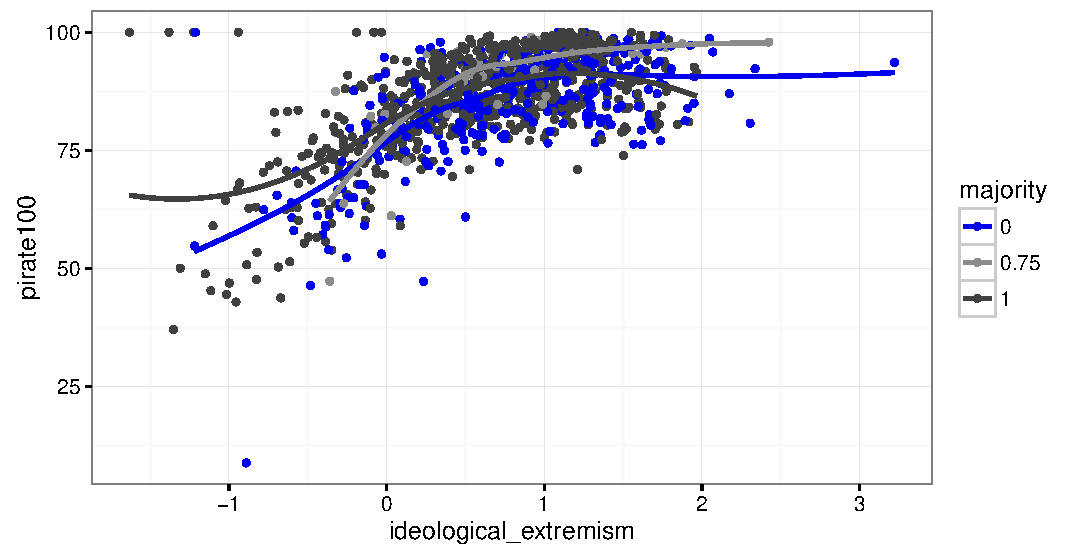
\includegraphics[width = \textwidth]{C:/Users/Ethan/Documents/GitHub/partycalls/plots/senate_lm_dem_iv-dv_majority.pdf}
\end{figure}

\begin{figure}[h]
	\caption{Main DV and Ideological Extremism - Southern and Other Democrats}
	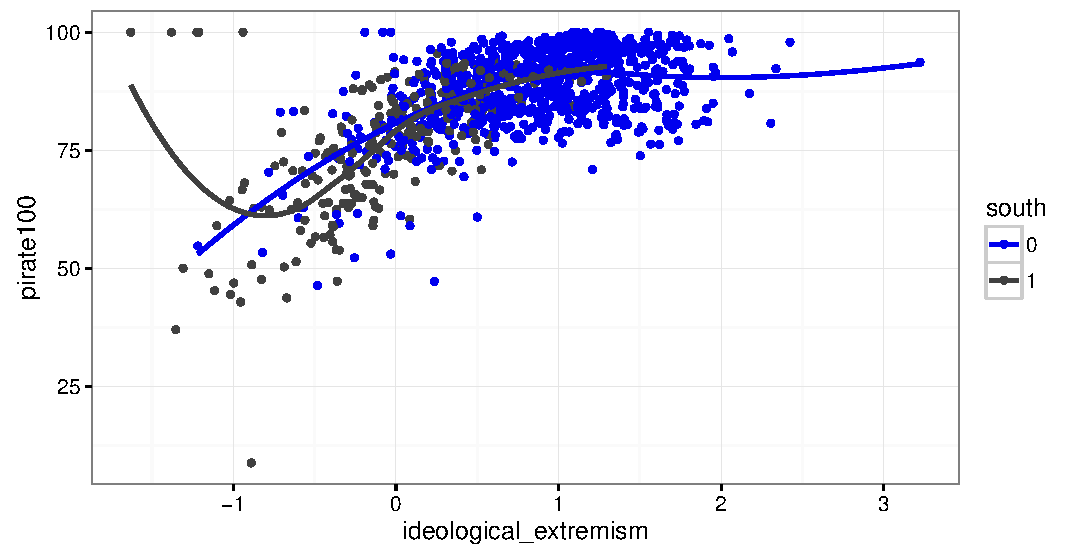
\includegraphics[width = \textwidth]{C:/Users/Ethan/Documents/GitHub/partycalls/plots/senate_lm_dem_iv-dv_south.pdf}
\end{figure}

\begin{figure}[h]
	\caption{Main DV and Ideological Extremism - Majority and Minority Party Republicans \textit{Note}: The light gray line and dots are for Congress 107.}
	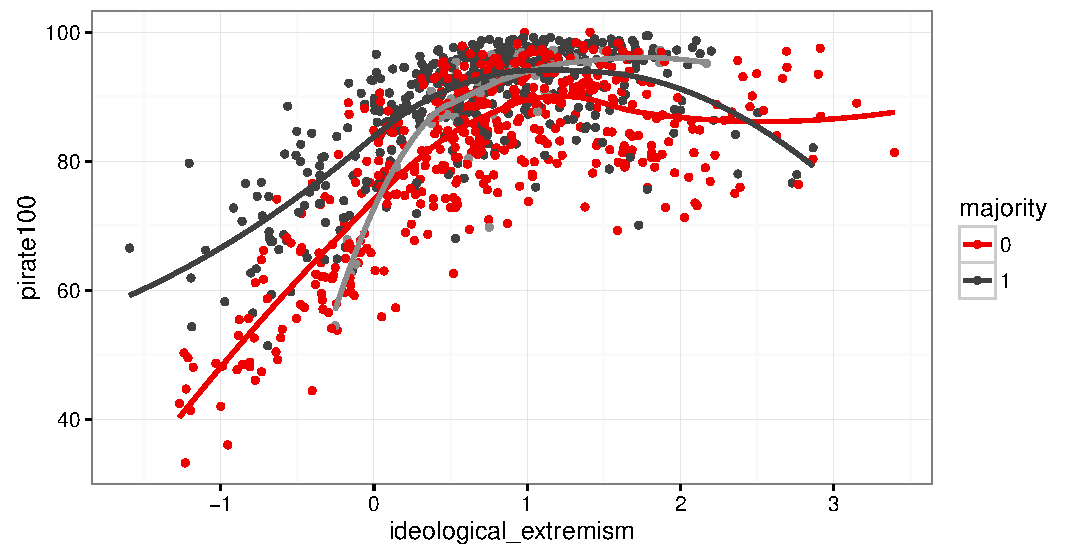
\includegraphics[width = \textwidth]{C:/Users/Ethan/Documents/GitHub/partycalls/plots/senate_lm_rep_iv-dv_majority.pdf}
\end{figure}

\begin{figure}[h]
	\caption{Main DV and Ideological Extremism - Southern and Other Republicans}
	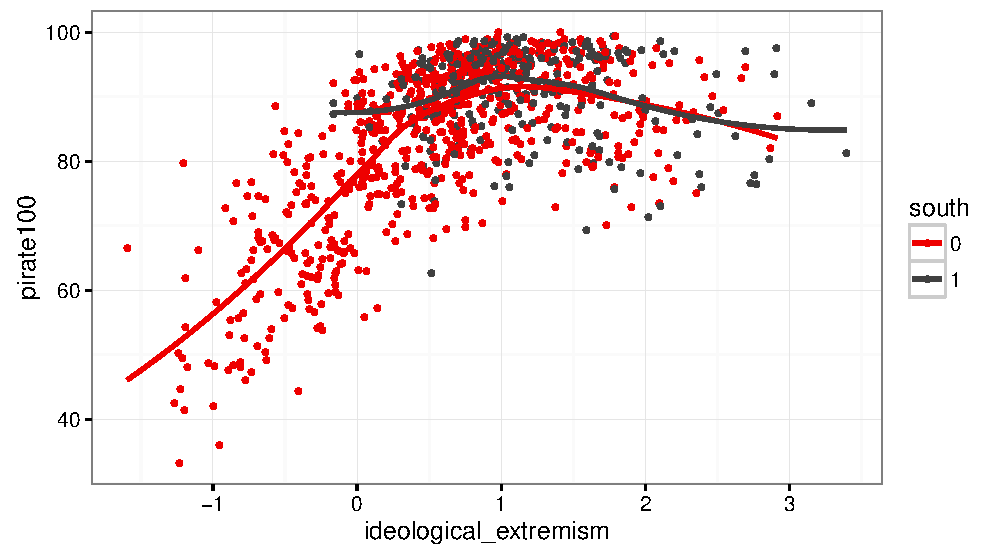
\includegraphics[width = \textwidth]{C:/Users/Ethan/Documents/GitHub/partycalls/plots/senate_lm_rep_iv-dv_south.pdf}
\end{figure}

\begin{figure}[h]
	\caption{Main DV and Ideological Extremism - Gingrich Senators and Other Republicans}
	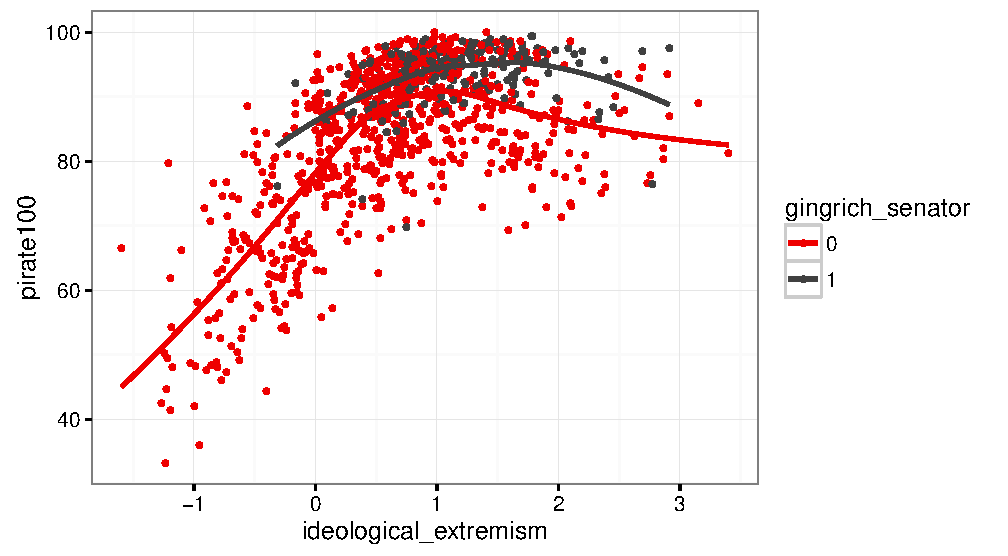
\includegraphics[width = \textwidth]{C:/Users/Ethan/Documents/GitHub/partycalls/plots/senate_lm_rep_iv-dv_gingrich.pdf}
\end{figure}

\begin{figure}[!htbp]
	\caption{IV IV Plot - Senate Majority and Minority Party Democrats \textit{Note}: The light gray line and dots are for Congress 107.}
	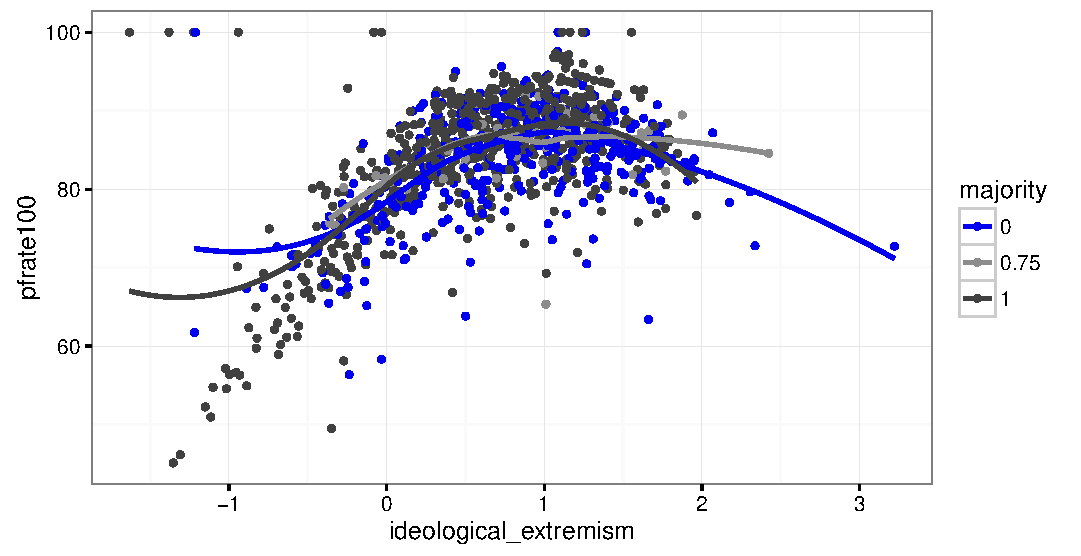
\includegraphics[width = \textwidth]{C:/Users/Ethan/Documents/GitHub/partycalls/plots/senate_lm_dem_iv_iv_majority.pdf}
\end{figure}

\begin{figure}[!htbp]
	\caption{IV IV Plot - Senate Southern and Other Democrats}
	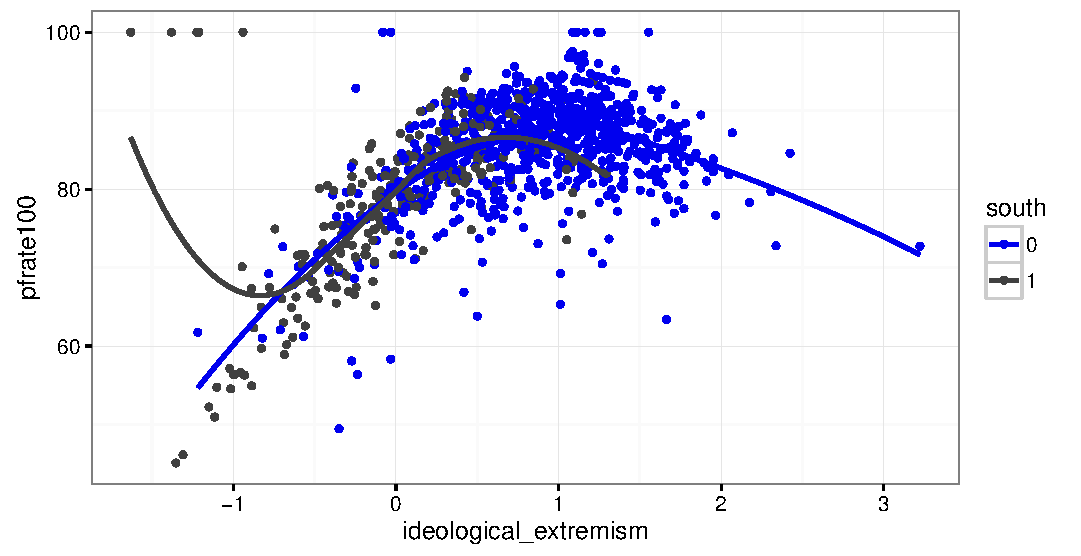
\includegraphics[width = \textwidth]{C:/Users/Ethan/Documents/GitHub/partycalls/plots/senate_lm_dem_iv_iv_south.pdf}
\end{figure}

\begin{figure}[!htbp]
	\caption{IV IV Plot - Senate Majority and Minority Party Republicans \textit{Note}: The light gray line and dots are for Congress 107.}
	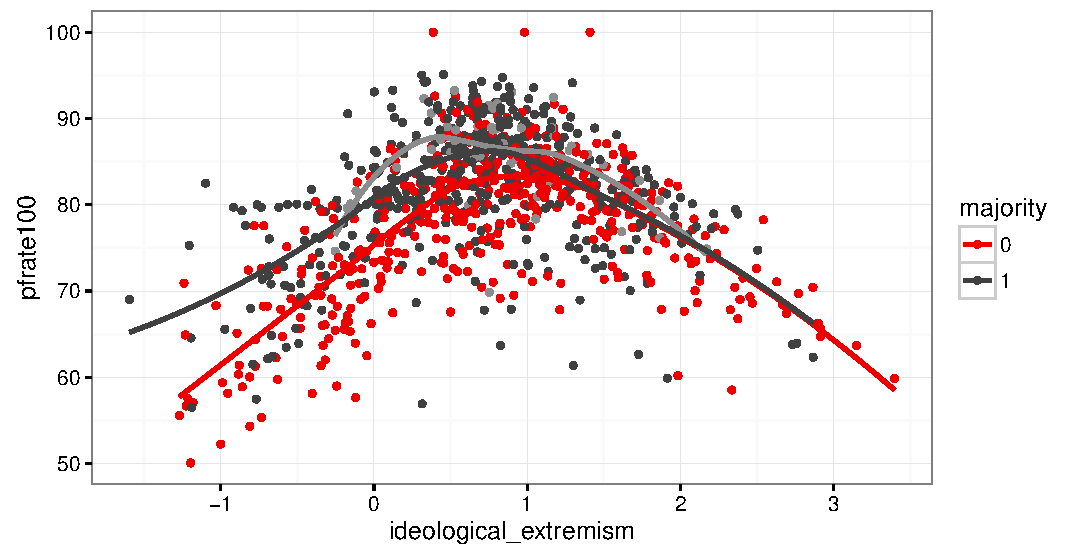
\includegraphics[width = \textwidth]{C:/Users/Ethan/Documents/GitHub/partycalls/plots/senate_lm_rep_iv_iv_majority.pdf}
\end{figure}

\begin{figure}[!htbp]
	\caption{IV IV Plot - Senate Southern and Other Republicans}
	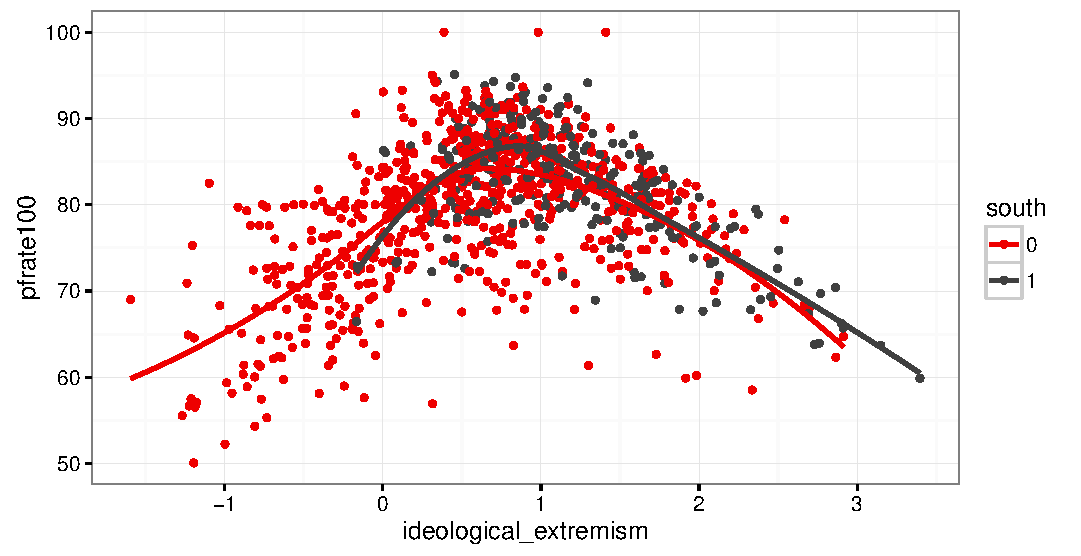
\includegraphics[width = \textwidth]{C:/Users/Ethan/Documents/GitHub/partycalls/plots/senate_lm_rep_iv_iv_south.pdf}
\end{figure}

\begin{figure}[!htbp]
	\caption{IV IV Plot - Gingrich Senators and Other Senate Republicans}
	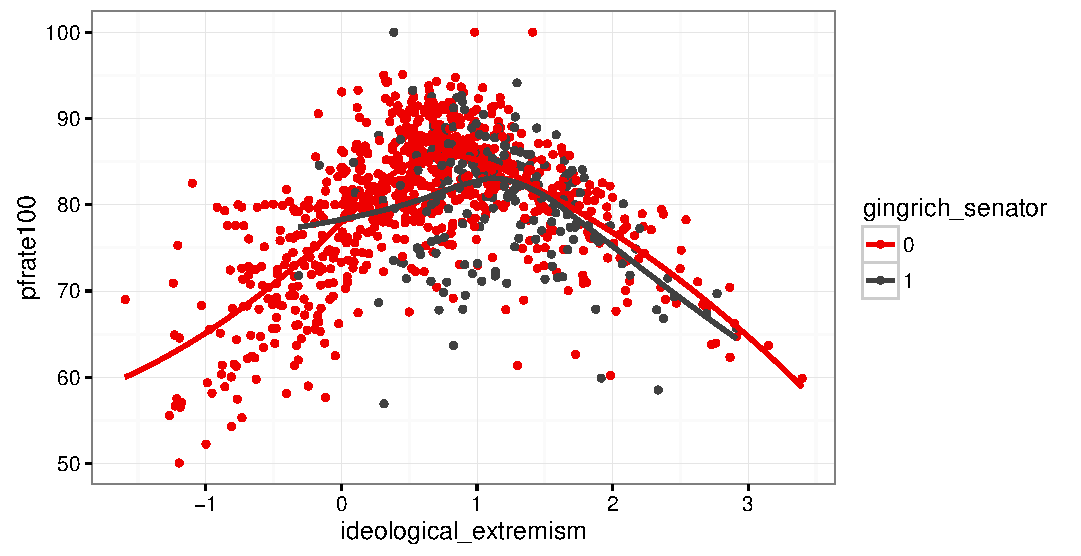
\includegraphics[width = \textwidth]{C:/Users/Ethan/Documents/GitHub/partycalls/plots/senate_lm_rep_iv_iv_gingrich.pdf}
\end{figure}

\begin{table}
	\begin{center}
		\caption{Full Regression Tables}
		\begin{tabular}{l c c c c }
			\hline
			& Democrats & Republicans & Majority & Minority \\
			\hline
			ideological\_extremism & $3.074^{***}$  & $7.831^{***}$   & $4.686^{***}$  & $7.923^{***}$ \\
			& $(0.411)$      & $(0.353)$       & $(0.316)$      & $(0.399)$     \\
			chair                  & $0.873$        & $3.807^{***}$   & $-0.141$       &               \\
			& $(0.543)$      & $(0.696)$       & $(0.521)$      &               \\
			pfrate100              & $0.757^{***}$  & $0.742^{***}$   & $0.705^{***}$  & $0.707^{***}$ \\
			& $(0.030)$      & $(0.031)$       & $(0.025)$      & $(0.035)$     \\
			pres vote share      & $24.184^{***}$ & $-14.698^{***}$ & $18.439^{***}$ & $-0.009$      \\
			& $(2.414)$      & $(3.062)$       & $(1.975)$      & $(3.196)$     \\
			south                  & $-1.636^{**}$  & $0.630$         & $0.146$        & $0.999$       \\
			& $(0.557)$      & $(0.574)$       & $(0.429)$      & $(0.623)$     \\
			power committee       & $-0.735$       & $0.461$         & $0.002$        & $-1.124$      \\
			& $(0.782)$      & $(0.924)$       & $(0.732)$      & $(1.079)$     \\
			vote share            & $-6.572^{**}$  & $16.428^{***}$  & $-2.189$       & $7.888^{**}$  \\
			& $(2.203)$      & $(2.822)$       & $(2.126)$      & $(2.990)$     \\
			female                 & $1.621^{*}$    & $0.345$         & $0.498$        & $4.148^{***}$ \\
			& $(0.732)$      & $(1.120)$       & $(0.761)$      & $(1.111)$     \\
			afam                   & $-0.483$       & $-10.167^{*}$   & $1.876$        & $-5.528$      \\
			& $(2.790)$      & $(4.234)$       & $(4.185)$      & $(3.215)$     \\
			latino                 & $1.835$        & $6.749^{*}$     & $4.800^{*}$    & $6.040$       \\
			& $(2.193)$      & $(2.750)$       & $(1.877)$      & $(3.507)$     \\
			up for reelection    & $-0.642$       & $-1.694^{**}$   & $-0.988^{*}$   & $-1.362^{*}$  \\
			& $(0.421)$      & $(0.531)$       & $(0.407)$      & $(0.601)$     \\
			seniority              & $-0.062$       & $0.104$         & $0.012$        & $0.146$       \\
			& $(0.060)$      & $(0.083)$       & $(0.067)$      & $(0.080)$     \\
			freshman               & $-1.533^{**}$  & $2.191^{**}$    & $-0.983$       & $0.876$       \\
			& $(0.574)$      & $(0.764)$       & $(0.570)$      & $(0.814)$     \\
			retiree                & $1.724$        & $2.385^{*}$     & $1.951^{*}$    & $2.617^{*}$   \\
			& $(0.912)$      & $(0.987)$       & $(0.866)$      & $(1.108)$     \\
			best committee        & $0.173$        & $-0.082$        & $-0.036$       & $0.298$       \\
			& $(0.129)$      & $(0.160)$       & $(0.124)$      & $(0.182)$     \\
			leader                 & $2.122^{**}$   & $1.270$         & $1.386^{*}$    & $1.965^{*}$   \\
			& $(0.719)$      & $(0.773)$       & $(0.668)$      & $(0.901)$     \\
			(Intercept)            & $12.019^{***}$ & $17.116^{***}$  & $18.262^{***}$ & $10.974^{**}$ \\
			& $(2.988)$      & $(3.600)$       & $(2.746)$      & $(4.131)$     \\
			\hline
			R$^2$                  & 0.690          & 0.650           & 0.684          & 0.616         \\
			Adj. R$^2$             & 0.685          & 0.644           & 0.679          & 0.609         \\
			Num. obs.              & 1039           & 949             & 1049           & 841           \\
			RMSE                   & 6.107          & 7.172           & 5.863          & 7.739         \\
			\hline
			\multicolumn{5}{l}{\scriptsize{$^{***}p<0.001$, $^{**}p<0.01$, $^*p<0.05$}}
		\end{tabular}
	\end{center}
\end{table}

\begin{figure}[h]
	\centering
	\caption{Senate lm Coefficient Plot}
	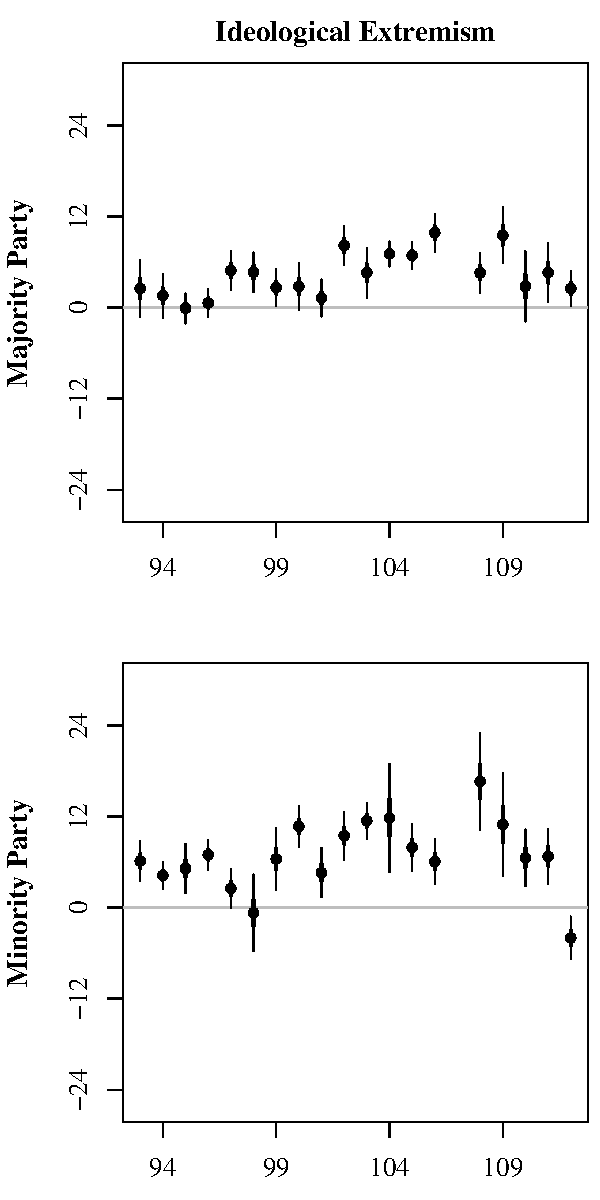
\includegraphics[width = 10cm]{C:/Users/Ethan/Documents/GitHub/partycalls/plots/senate-figure2-lm.pdf}
\end{figure}











\end{document}